% !TEX root = ../p344-xie.tex 
In this section, we design experiments to empirically (1) validate that \errorname correlates with Deviation and (2)~evaluate the effectiveness of \systemname compression.

We use two specific datasets in the experiment: (1) SQL query logs of the Google+ Android app extracted from the PocketData public dataset~\cite{DBLP:conf/tpctc/KennedyACZ15} and (2) SQL query logs that capture all query activity on the majority of databases at a major US bank over a period of approximately 19 hours.
A summary of these two datasets is given in Table~\ref{table:datasummary}.

\begin{table}
\centering
\bfcaption{Summary of Data sets}
\label{table:datasummary}
{\small \centering
\begin{tabular}{c c c}
\toprule
Statistics & PocketData & US bank \\
\midrule
\# Queries & 629582& 1244243\\
\midrule
\# Distinct queries & 605& 188184\\
\midrule
\# Distinct queries (w/o const)& 605& 1712\\
\midrule
\# Distinct conjunctive queries & 135& 1494\\
\midrule
\# Distinct re-writable queries & 605& 1712\\
\midrule
Max query multiplicity & 48651 & 208742\\
\midrule
\# Distinct features & 863& 144708\\
\midrule
\# Distinct features (w/o const) & 863& 5290\\
\midrule
Average features per query & 14.78& 16.56\\
\bottomrule
\end{tabular}
}
\trimfigurewhitespace
\end{table}

\begin{figure*}[h!]
	\captionsetup[subfigure]{justification=centering}
    \centering
    \begin{subfigure}[b]{0.48\textwidth}
        \centering
        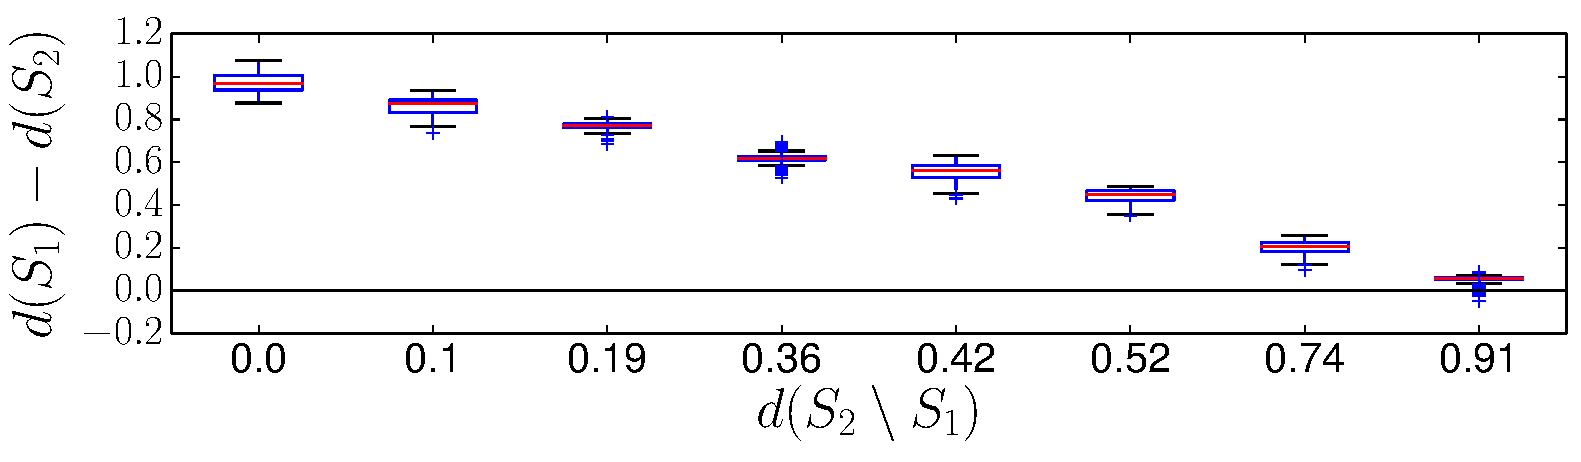
\includegraphics[width=\textwidth]{QueryLogSummarization/graphics/ContainmentCapturesDeviation_BankData.pdf}
        \bfcaption{Containment captures Deviation (US bank)}
        \label{fig:containmentcapturesdeviation_bankdata}
    \end{subfigure}
        ~
    \begin{subfigure}[b]{0.48\textwidth}
        \centering
        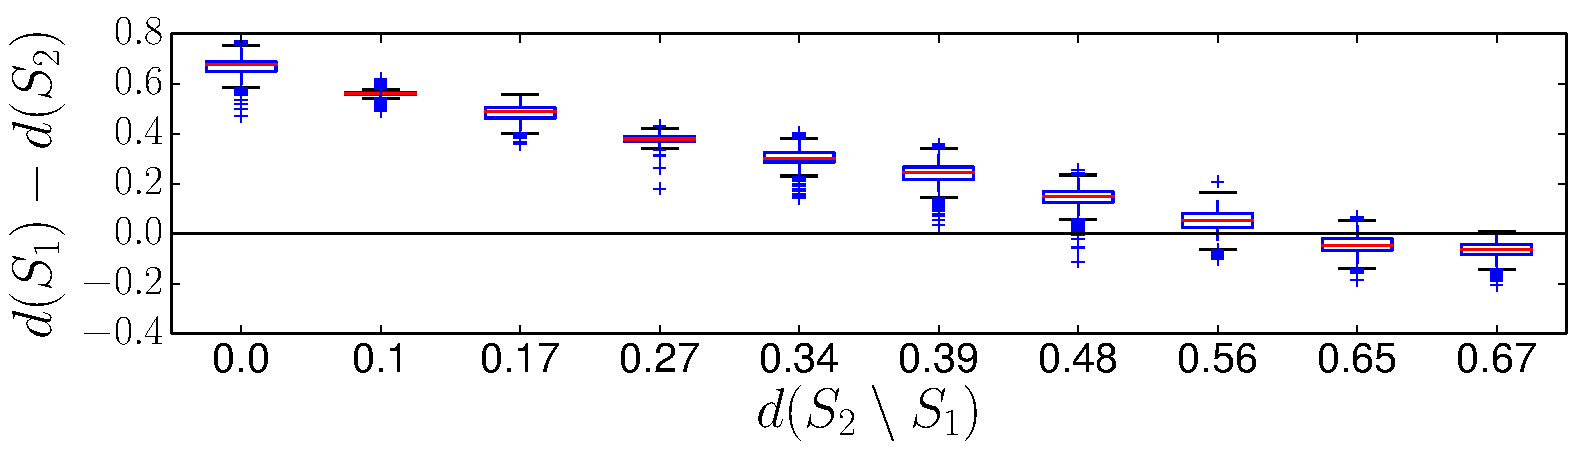
\includegraphics[width=\textwidth]{QueryLogSummarization/graphics/ContainmentCapturesDeviation_PocketData.pdf}
        \bfcaption{Containment captures Deviation (PocketData)}
        \label{fig:containmentcapturesdeviation_pocketdata}
    \end{subfigure}
    ~
    \begin{subfigure}[b]{0.485\textwidth}
        \centering
         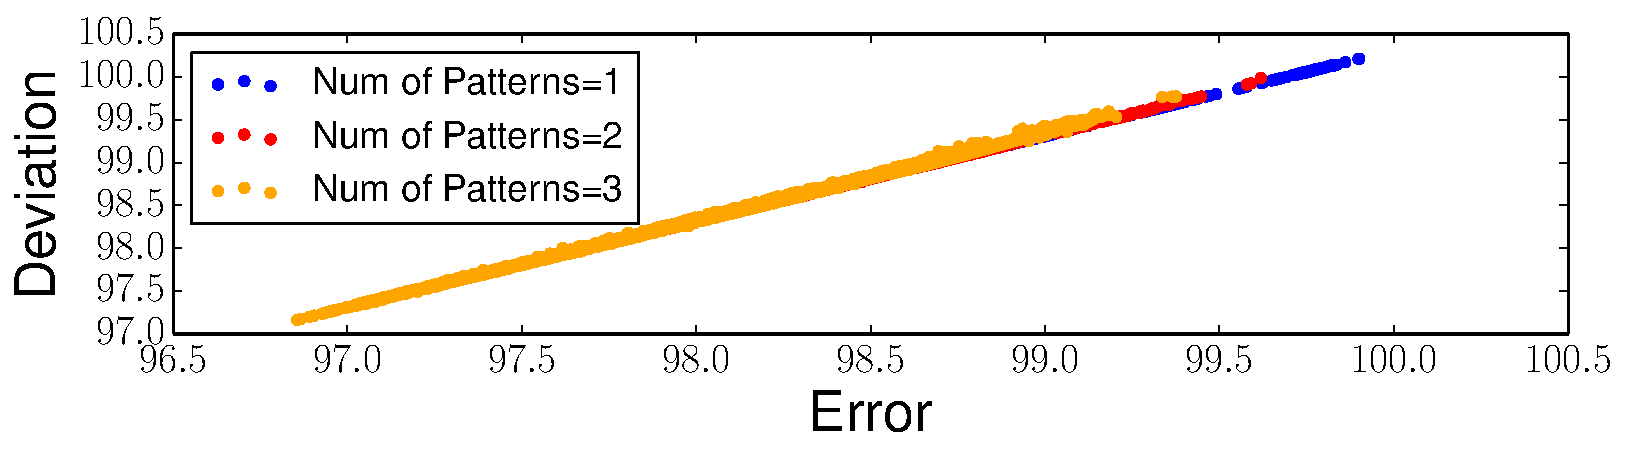
\includegraphics[width=\textwidth]{QueryLogSummarization/graphics/ErrorCapturesDeviation_BankData.pdf}
        \bfcaption{Error captures Deviation (US bank)}
        \label{fig:errorcapturesdeviation_bankdata}
    \end{subfigure}
        ~
    \begin{subfigure}[b]{0.485\textwidth}
        \centering
        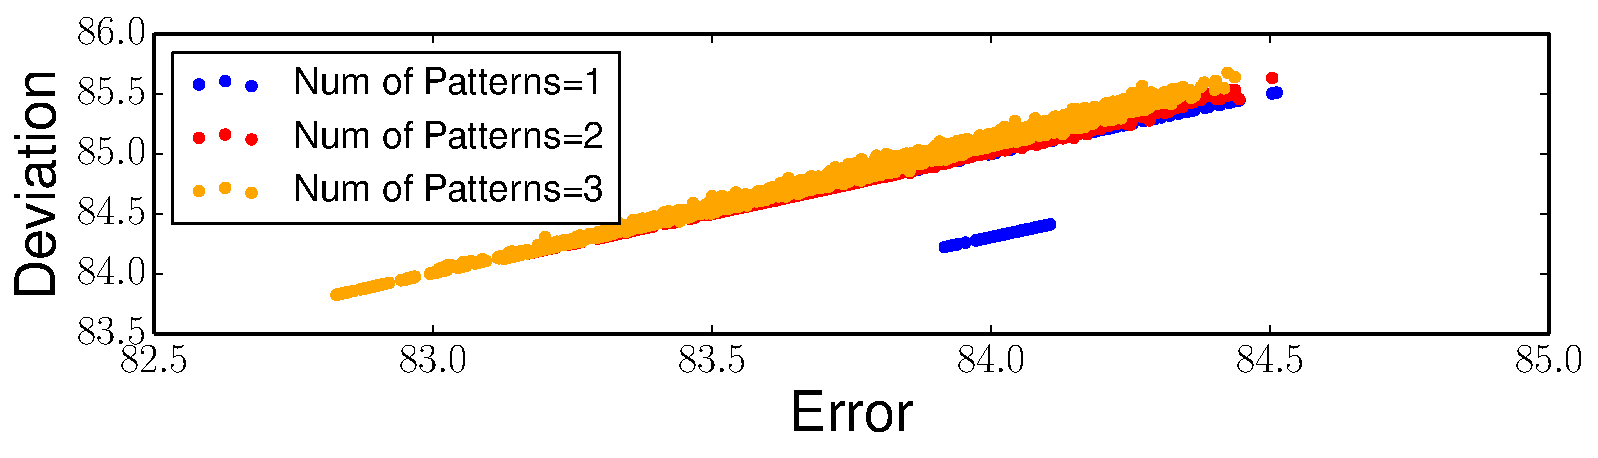
\includegraphics[width=\textwidth]{QueryLogSummarization/graphics/ErrorCapturesDeviation_PocketData.pdf}
        \bfcaption{Error captures Deviation (PocketData)}
        \label{fig:errorcapturesdeviation_pocketdata}
    \end{subfigure}
    ~
%     \begin{subfigure}[b]{0.45\textwidth}
%        \centering
%        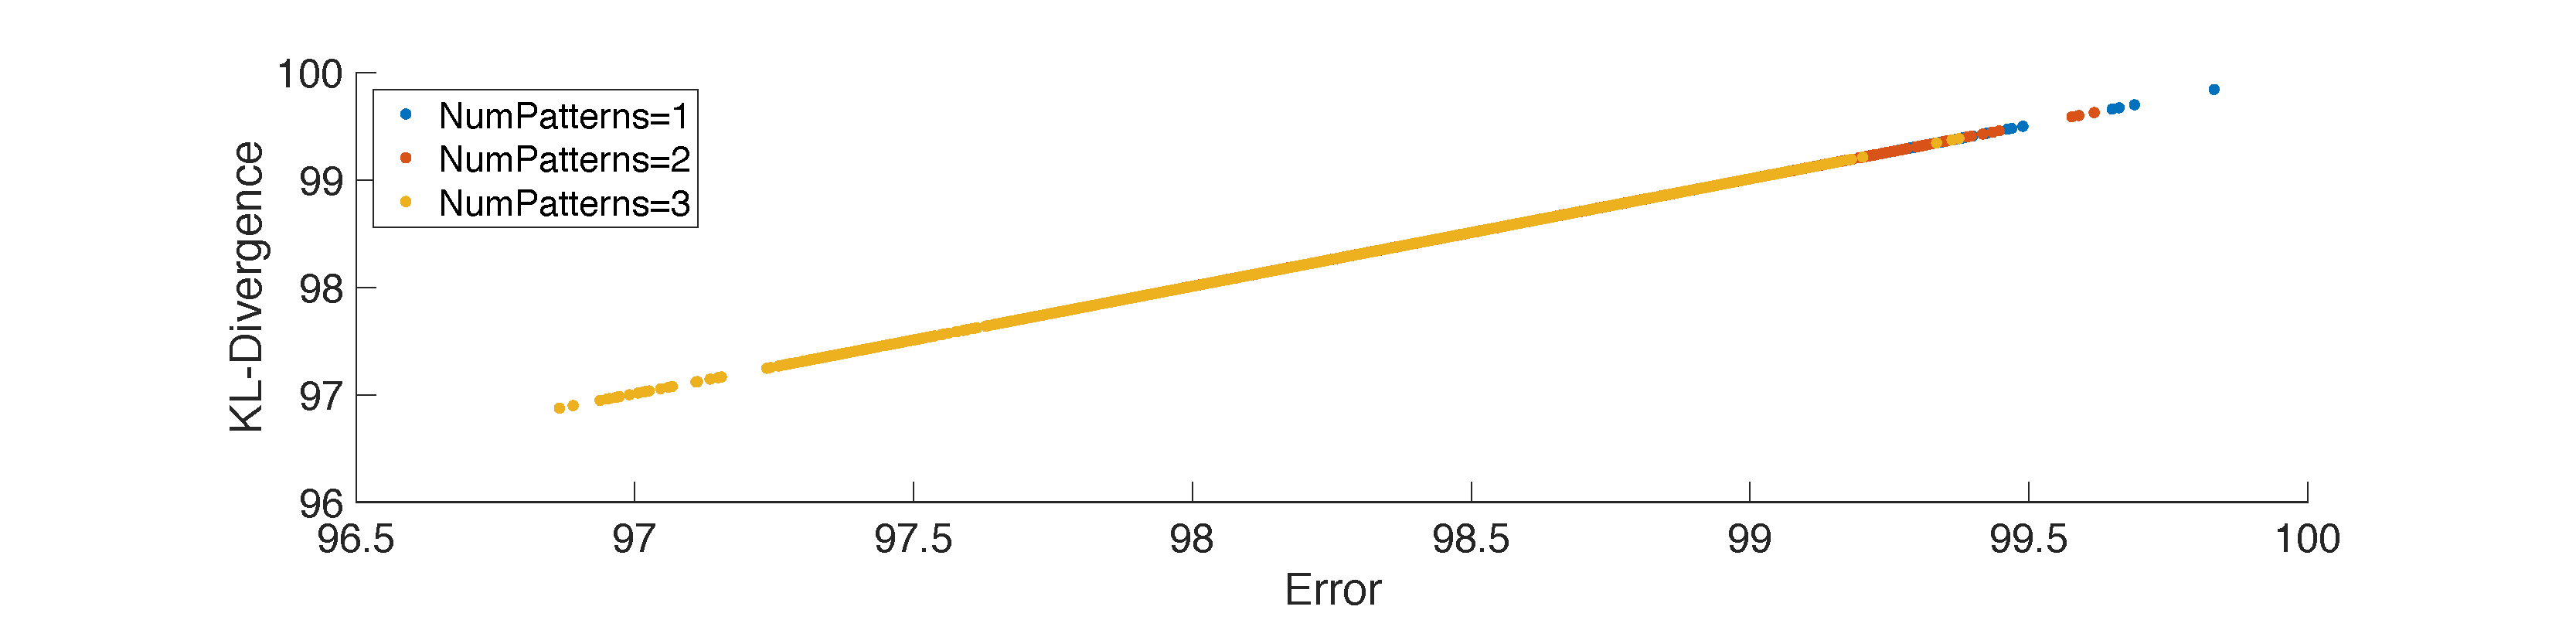
\includegraphics[width=\textwidth]{graphics/ErrorCapturesKL_BankData.pdf}
%        \bfcaption{Error captures KL-divergence (US bank)}
%        \label{fig:errorcapturesKL_bankdata}
%\end{subfigure}
%    ~
%     \begin{subfigure}[b]{0.45\textwidth}
%        \centering
%        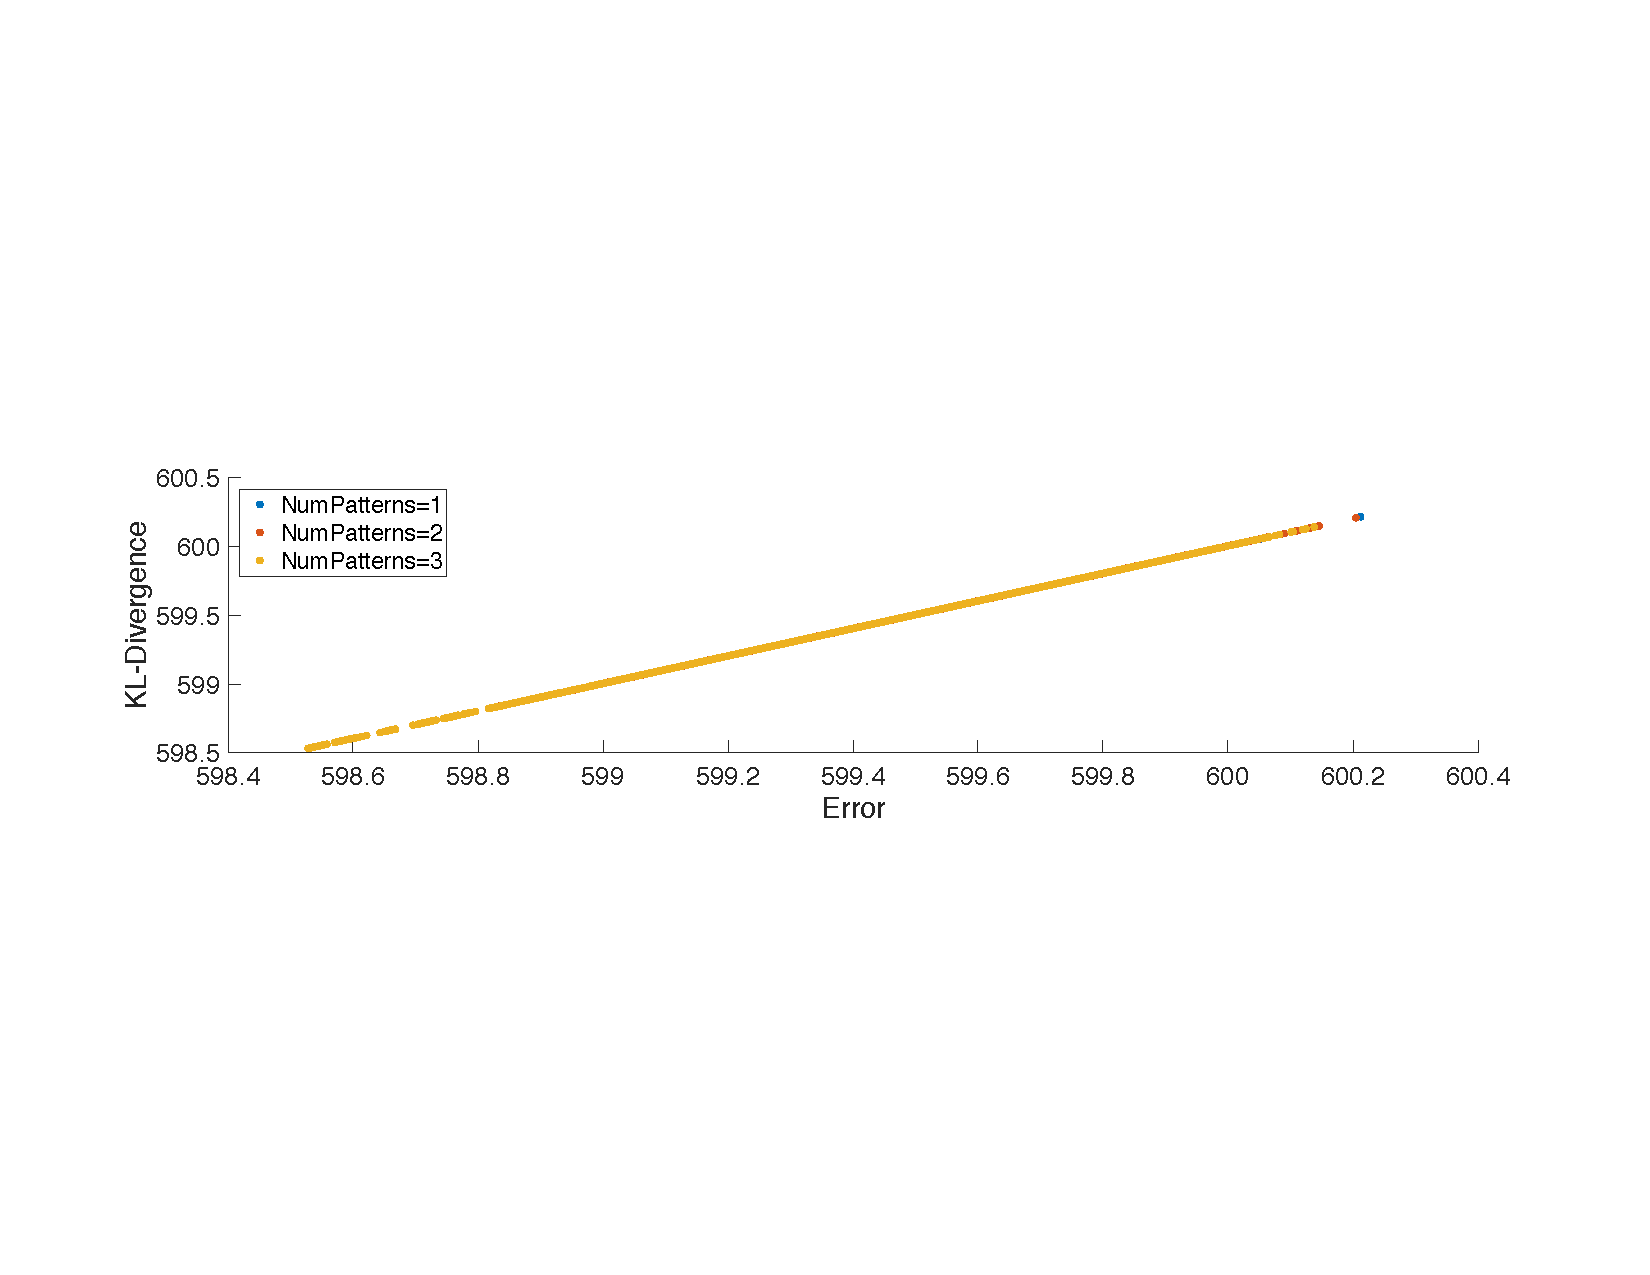
\includegraphics[width=\textwidth]{graphics/ErrorCapturesKL_PocketData.pdf}
%        \bfcaption{Error captures KL-divergence (PocketData)}
%        \label{fig:errorcapturesKL_pocketdata}
%\end{subfigure}
%    ~
     \begin{subfigure}[b]{0.48\textwidth}
        \centering     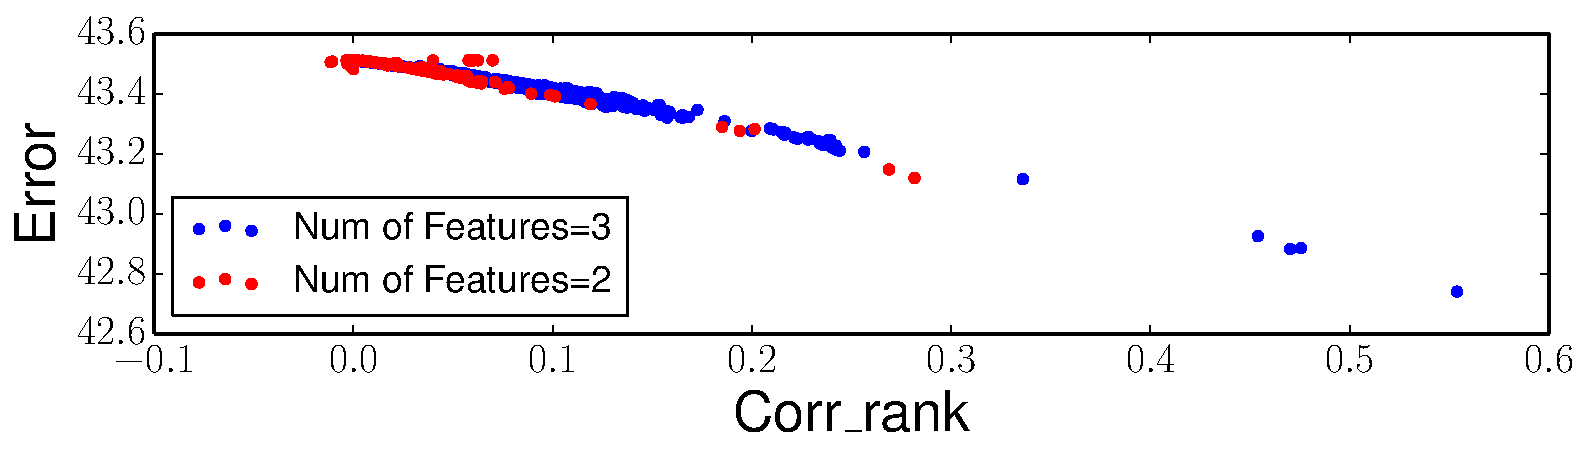
\includegraphics[width=\textwidth]{QueryLogSummarization/graphics/ErrorCapturesCorrelation_BankData.pdf}
        \bfcaption{Error captures Correlation (US bank)}
        \label{fig:errorcapturescorrelation_bankdata}
\end{subfigure}
    ~
     \begin{subfigure}[b]{0.48\textwidth}
        \centering     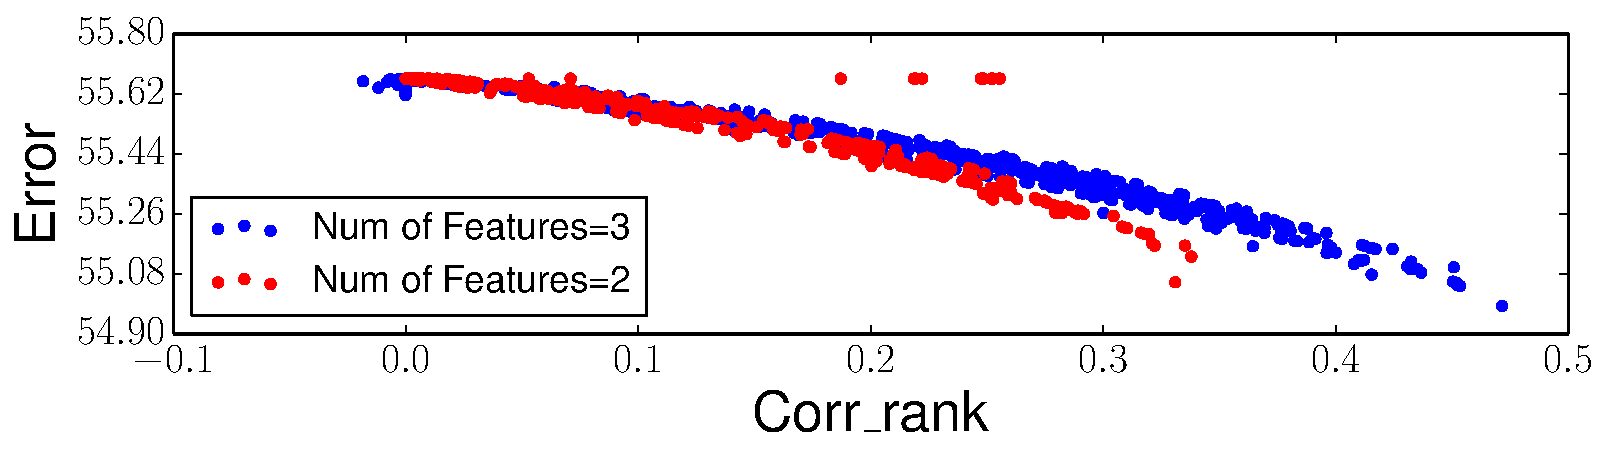
\includegraphics[width=\textwidth]{QueryLogSummarization/graphics/ErrorCapturesCorrelation_PocketData.pdf}
        \bfcaption{Error captures Correlation (PocketData)}
        \label{fig:errorcapturescorrelation_pocketdata}
\end{subfigure}
    
\bfcaption{Validating \Errorname}
\label{fig:validatingencodingerror}
\trimfigurewhitespace
\end{figure*}

\tinysection{The PocketData-Google+ query log} The dataset consists of SQL logs that capture all database activities of 11 Android phones. 
We selected the Google+ application for our study since it is one of the few applications where all users created a workload. 
This dataset is a stable workload of exclusively machine-generated queries.

\tinysection{The US bank query log}
This log is an anonymized record of queries processed by multiple relational database servers at a major US bank~\cite{DBLP:conf/www/KulLXCCKU16} over a period of 19 hours.
Of the nearly 73 million database operations captured, 58 million are not directly queries, but rather invocations of stored procedures.
A further 13 million used non-standard SQL features not supported by our SQL parser. 
Of the remaining of the 2.3 million parsed SQL queries, we base our analysis on the 1.25 million conjunctive \texttt{SELECT} queries. 
This dataset can be characterized as a diverse workload of both machine- and human-generated queries.

\tinysection{Common Experiment Settings}
\label{sec:commonexperimentsettings}
Experiments were performed on a 2.8 GHz Intel Core i7 CPU with 16 GB 1600 MHz DDR3 memory and a SSD running macOS Sierra.

\tinysection{Constant Removal}
A number of queries in the US bank query log differ only in hard-coded constant values.
Table~\ref{table:datasummary} shows the total number of queries, as well as the number of distinct queries if we ignore constants.
By comparison, queries in PocketData all use JDBC parameters.
For these experiments, we ignore constant values in queries.

\tinysection{Query Regularization}
We apply query rewrite rules (same as \cite{8352666}) to regularize queries into equivalent conjunctive forms, where possible. 
Table~\ref{table:datasummary} shows that $\frac{135}{605}$ and $\frac{1494}{1712}$ of distinct queries are in conjunctive form for PocketData and US bank respectively. 
After regularization, all queries in both data sets can be either simplified into conjunctive queries or re-written into a \texttt{UNION} of conjunctive queries compatible with feature scheme of Aligon et al.~\cite{DBLP:journals/kais/AligonGMRT14}.

\tinysection{Convex Optimization Solving}
All convex optimization problems for measuring \errorname and Deviation are solved by the \textit{successive approximation heuristic} implemented by the CVX toolbox~\cite{cvx} with the Sedumi solver.

\subsection{Validating \Errorname}
\label{sec:motivateencodingerror}
In this section, we validate that \errorname is a practical alternative to Deviation.
In addition, we also offer measurements on its correlation with Deviation and score $corr\_rank$ in Section~\ref{sec:naivemixtureencodingrefinement}.
%
As it is impractical to enumerate all possible encodings, we choose a subset of encodings for both datasets. 
Specifically, we first select all features with frequencies in the range $[0.01,0.99]$ and use these features to construct patterns.
We then enumerate combinations of $K$ (up to 3) patterns as our chosen encodings.

\tinysection{Containment Captures Deviation}
Here we empirically verify that containment (Section~\ref{sec:validateencodingerror}) captures Deviation (i.e., $\encoding_1\leq_{\Omega} \encoding_2\to d(\encoding_1)\leq d(\encoding_2)$) to complete the chain of reasoning that \errorname captures Deviation.
Figures~\ref{fig:containmentcapturesdeviation_bankdata} and \ref{fig:containmentcapturesdeviation_pocketdata} show all pairs of encodings where $\encoding_2\supset \encoding_1$.
The y-axis shows the difference in Deviation values (i.e., $d(\encoding_2)-d(\encoding_1)$).
Deviation $d(\encoding)$ is approximated by drawing 1 million samples from the space $\Omega_{\encoding}$ induced by the encoding $\encoding$.
For clarity, we bin pairs of encodings by the degree of overlap between them, measured by the Deviation of the set-difference $d(\encoding_2\setminus \encoding_1)$; Higher $d(\encoding_2\setminus \encoding_1)$ implies less overlap. 
Y-axis values are grouped into bins and visualized by boxplot where the boxes represent ranges within standard deviation and crosses are outliers.
Intuitively, \emph{points above zero} on the y-axis (i.e., $d(\encoding_2)-d(\encoding_1) > 0$) are pairs of encodings where the Deviation order agrees with containment order.
This is the case for virtually all encoding pairs.  

\tinysection{Additive Separability of Deviation}
We also observe from Figures~\ref{fig:containmentcapturesdeviation_bankdata} and ~\ref{fig:containmentcapturesdeviation_pocketdata} that agreement between Deviation and containment order is correlated with overlap: More similar encodings are more likely to have agreement.
Combined with Proposition~\ref{prop:monotone}, this shows first that for similar encodings, \errorname is likely to be a reliable indicator of Deviation.
This also suggests that Deviation is additively separable: The information loss (i.e., $d(\encoding_2)-d(\encoding_1)$) caused by excluding the encoding $\encoding_2\setminus \encoding_1$ from $\encoding_2$ correlates with the quality (i.e., $d(\encoding_2\setminus \encoding_1)$) of the encoding $\encoding_2\setminus \encoding_1$ itself:\vspace*{-4mm}

{\small
$$\encoding_2\supset \encoding_1\to d(\encoding_2)-d(\encoding_1)<0\hspace{5mm}\text{and}\hspace{5mm}d(\encoding_2\setminus \encoding_1)\propto d(\encoding_2)-d(\encoding_1)$$ 
}\vspace*{-5mm}

\tinysection{Error correlates with Deviation}
As a supplement, Figures~\ref{fig:errorcapturesdeviation_bankdata} and ~\ref{fig:errorcapturesdeviation_pocketdata} empirically confirm that that \errorname (x-axis) indeed closely correlates with Deviation (y-axis).
Mirroring our findings above, correlation between them is tighter at lower \errorname.

%\tinysection{Error Correlates With KL-Divergence}
%Figures~\ref{fig:errorcapturesKL_bankdata} and ~\ref{fig:errorcapturesKL_pocketdata} show the relationship between \errorname (x-axis) and KL-Divergence between the true distribution $\rho^*$ and the space representative distribution $\overline{\rho}_S$ (y-axis), as discussed in Section~\ref{sec:maximumentropydistribution}. The two are tightly correlated.

\tinysection{Error and Feature-Correlation}
Figure~\ref{fig:errorcapturescorrelation_bankdata} and ~\ref{fig:errorcapturescorrelation_pocketdata} show the relationship between \errorname (y-axis) and score $corr\_rank$ (x-axis), as discussed in Section~\ref{sec:naivemixtureencodingrefinement}. Values of y-axis are \errorname of the naive encodings extended by a non-naive pattern $\vec{b}$ containing multiple features (up to 3 for illustrative purposes). 
One can observe that \errorname of extended naive encodings almost linearly correlates with $corr\_rank(\vec b)$. 
In addition, one can also observe that $corr\_rank$ becomes higher when the pattern $\vec{b}$ encodes more correlated features. 

\subsection{Feature-Correlation Refinement}
\label{sec:motivatepatternmixturesummaries}
In this section, we design experiments serving two purposes: (1) Evaluating the potential reduction of Error from refining naive mixture encodings through state-of-the-art pattern-based summarizers, and (2) Evaluating whether we can replace naive mixture encodings by the encodings created from summarizers that we have plugged-in.

\hyphenation{Laser-light}

\tinysection{Experiment Setup}
To serve both purposes, we construct pattern mixture encodings under three configurations: (1)~Naive mixture encodings; (2)~Pattern-based encodings and (3)~Naive mixture encodings refined into pattern-based encodings.
Naive mixture encodings are constructed by K-Means clustering. 
Pattern-based encodings are generated by two state-of-the-art pattern-based summarizers: 
(1)~\textit{Laserlight}~\cite{DBLP:journals/pvldb/GebalyAGKS14} that summarizes multi-dimensional data in order to predict an augmented binary variable and 
(2)~\textit{MTV}~\cite{DBLP:journals/tkdd/MampaeyVT12} that aims at mining maximally informative patterns that summarize binary multi-dimensional data. 
%Detailed descriptions and experiment configurations of these two algorithms are given in Appendix~\ref{appendix:experimentsettingsforpatternbasedalgorithms}.

The experimental results are shown in Figure~\ref{fig:motivatenaivemixtureencodings_bankdata} that contains 3 sub-figures sharing the same x-axis, i.e., the number of clusters.
Figure~\ref{fig:PatternMixtureEncodingErrorComparisonAlone_bankdata} compares the Error (y-axis) between naive mixture encodings and pattern mixture encodings that consist of patterns mined from \textit{MTV} or \textit{Laserlight}.
Figure~\ref{fig:PatternMixtureEncodingErrorComparisonPiggybacking_bankdata} evaluates the change in Error (y-axis) through refining naive mixture encodings by adding patterns from \textit{MTV} or \textit{Laserlight}.
Figure~\ref{fig:mixtureencodingsrunningtimecomparison_bankdata} compares the runtime (y-axis) between constructing naive mixture encodings and applying \textit{MTV} or \textit{Laserlight}.
We only show the results for US bank query log as results for PocketData give similar observations. 

\subsubsection{Pattern-based vs Naive Mixture Encodings}
\label{sec:Replacing_Naive_Mixture_Encodings}
Figure~\ref{fig:PatternMixtureEncodingErrorComparisonAlone_bankdata} and~\ref{fig:mixtureencodingsrunningtimecomparison_bankdata} suggest that naive mixture encodings outperform pattern-based encodings in two ways.

\tinysection{\errorname}
We observe from Figure~\ref{fig:PatternMixtureEncodingErrorComparisonAlone_bankdata} that the \errorname of naive mixture encodings are orders of magnitude lower than pattern-based encodings generated by \textit{Laserlight} or \textit{MTV} alone.
%Note that the curve of MTV overlaps with that of Laserlight.

\tinysection{Computation Efficiency}
From Figure~\ref{fig:mixtureencodingsrunningtimecomparison_bankdata} we observe that the runtime of constructing naive mixture encodings is significantly lower than that of \textit{Laserlight} and \textit{MTV}.

The one way where pattern-based encodings outperform naive mixture encodings is in Total Verbosity. 
\textit{Laserlight} and \textit{MTV} produce encodings with significantly fewer patterns, as the naive mixture encoding requires at least one pattern for each feature (e.g., 5290 patterns in the US bank query log).
Conversely, mining this number of patterns is computationally infeasible (Figure~\ref{fig:mixtureencodingsrunningtimecomparison_bankdata}).



% is partially due to the lower verbosity of their result than \textit{naive mixture encoding}.
% More specifically, recall that the Total Verbosity of \textit{naive mixture encoding} is the sum over the number of distinct features in each cluster.
% In Figure~\ref{fig:PatternMixtureEncodingErrorComparisonAlone_bankdata}, the Total Verbosity of the \textit{naive mixture encoding} can be as large as $5000$ for the US bank data set (See Figure~\ref{fig:TotalVerbosityVNumCluster}).
% Due to computation efficiency (see ),  it is not practical to set up the number of patterns to be mined from \textit{Laserlight} and \textit{MTV} the same as \textit{naive mixture encoding} in our experiments.

\begin{figure}[ht!]
	\captionsetup[subfigure]{justification=centering}
    \centering
    \begin{subfigure}[b]{0.47\textwidth}
      \centering       
      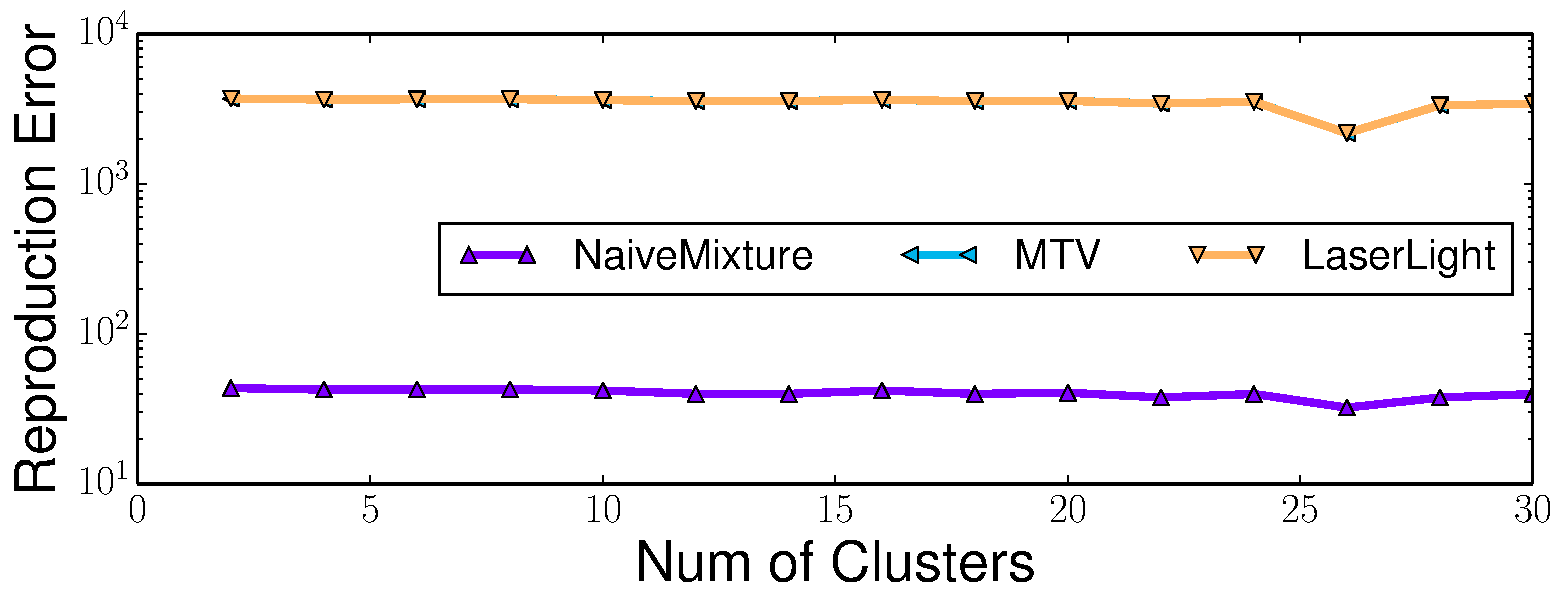
\includegraphics[width=\textwidth]{QueryLogSummarization/graphics/PatternMixtureSummaryErrorComparisonAlone_bankdata.pdf}
     \bfcaption{Naive Mixture v. LaserLight/MTV alone. Note that y-axis is in log scale.}     \label{fig:PatternMixtureEncodingErrorComparisonAlone_bankdata}
    \end{subfigure}
    ~
    \begin{subfigure}[b]{0.47\textwidth}
        \centering       
        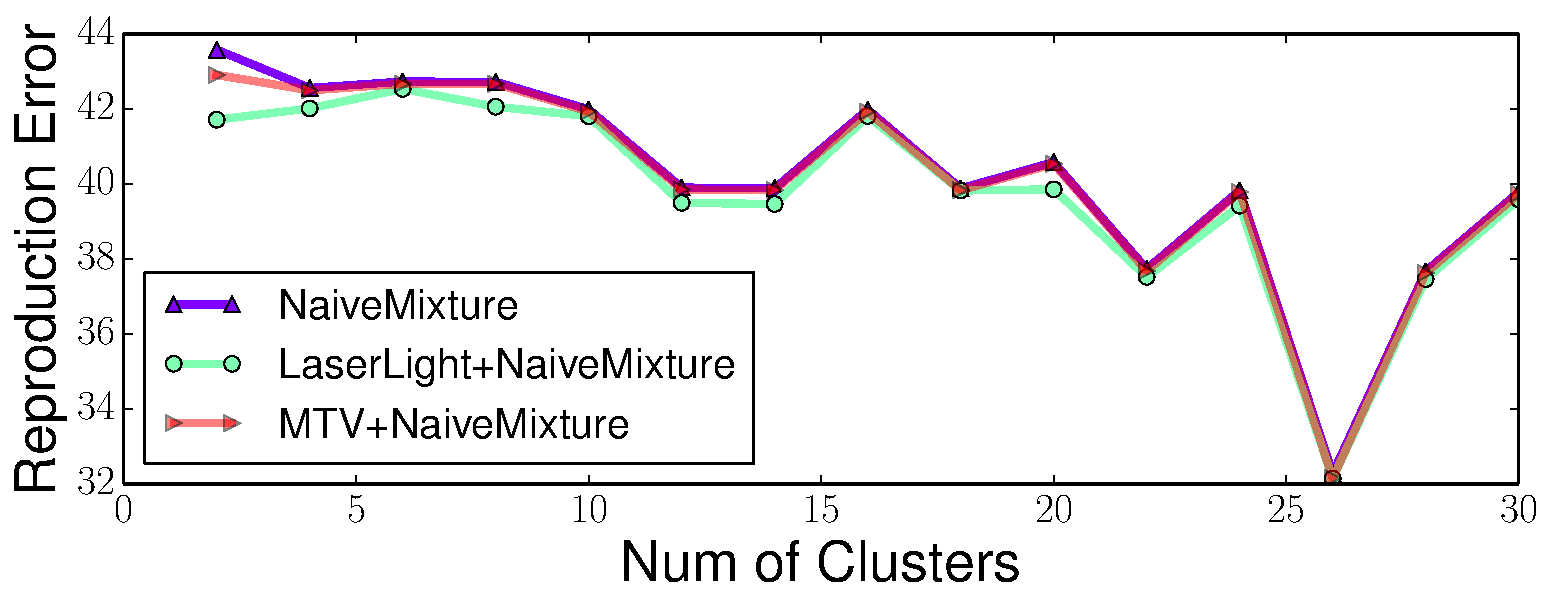
\includegraphics[width=\textwidth]{QueryLogSummarization/graphics/PatternMixtureSummaryErrorComparisonPiggybacking_bankdata.pdf}
     \bfcaption{Naive Mixture v. Naive Mixture+LaserLight/MTV. Note that we offset y-axis (non-zero start).}      \label{fig:PatternMixtureEncodingErrorComparisonPiggybacking_bankdata}
    \end{subfigure}
    ~
    \begin{subfigure}[b]{0.47\textwidth}
    \centering       
    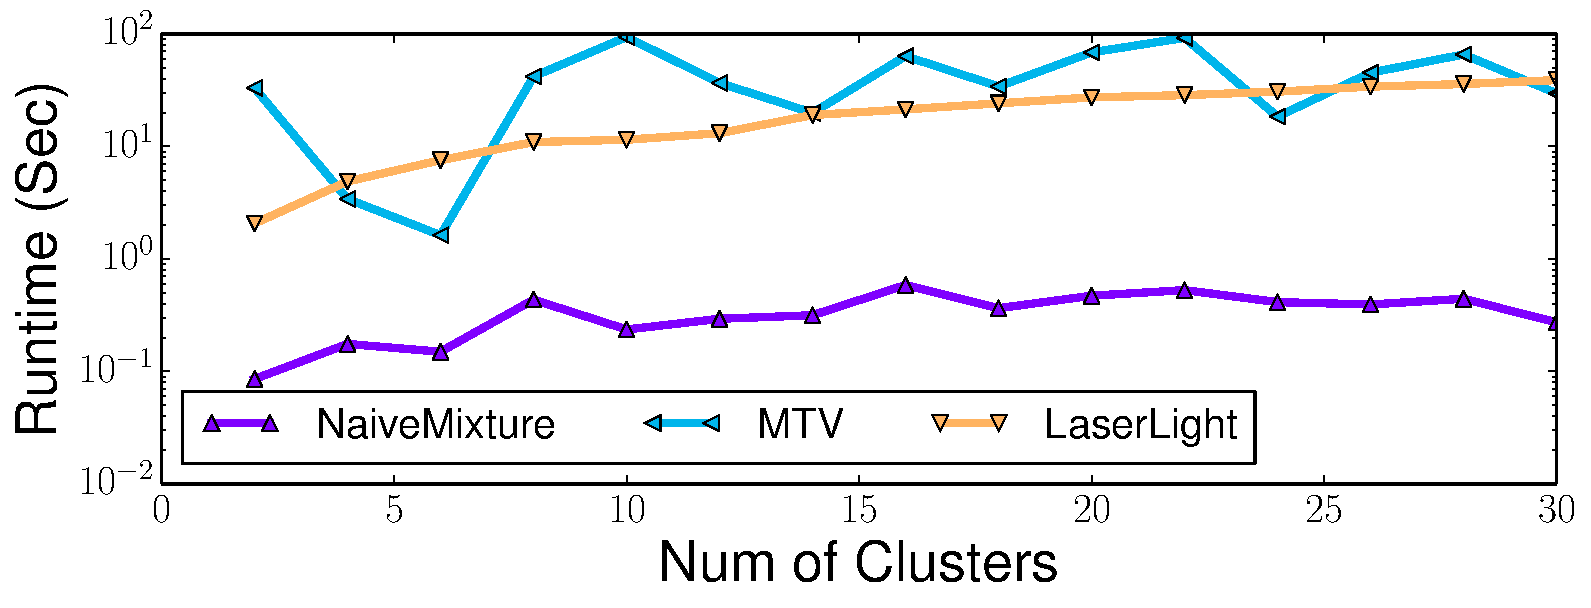
\includegraphics[width=\textwidth]{QueryLogSummarization/graphics/PatternMixtureSummaryRunningTime_bankdata.pdf}
    \bfcaption{Runtime Comparison (y-axis in log scale)}   
    \label{fig:mixtureencodingsrunningtimecomparison_bankdata}
    \end{subfigure}
\bfcaption{Feature-correlation refinement (US bank)}   \label{fig:motivatenaivemixtureencodings_bankdata}
\trimfigurewhitespace
\end{figure}

\subsubsection{Refining Naive Mixture Encodings}
\label{sec:refiningnaivemixtureencodings}
The experiment result is shown in Figure~\ref{fig:PatternMixtureEncodingErrorComparisonPiggybacking_bankdata}.
Note that we offset y-axis to show the change in Error.
We observe from the figure that reduction of Error contributed by plugging-in pattern-based summarizers is small for both algorithms.

\tinysection{Dimensionality Restriction}
For \textit{Laserlight}, the observation is partially due to the fact that we only keep top $100$ features (in terms of variability) of the data as its input, since \textit{Laserlight} is implemented in PostgresSQL 9.1 which has a threshold of $100$ arguments (one argument for each feature) that can be passed to a function.

\tinysection{Pattern Restriction}
For \textit{MTV}, this is due to a runtime error that limits us to $15$ or less patterns.
We refer the reader to Section 4.5 in~\cite{DBLP:journals/tkdd/MampaeyVT12} that explains the difficulty in inferring the maximum entropy distribution constrained by a large number of non-naive patterns.

% \tinysection{Anti-Correlation}
% The major source of Error for summarizing both data sets is \textit{mutual exclusiveness}, a type of anti-correlation that cannot be effectively reduced by pattern based summarizers.
% To illustrate, consider the following example queries in the log.
% \begin{lstlisting}
%  SELECT _time,_id FROM Messages WHERE _time>20
%  SELECT _time,_id FROM Messages WHERE _time>30
% \end{lstlisting}
% Example queries differ in right hand side (RHS) of the filtering condition in \texttt{WHERE} clause.
% Since the RHS can be assigned only one value, the set of possible RHS values translate to \textit{mutually exclusive} features. 
% Encoding mutual exclusiveness among those features requires potentially large number of patterns mined from pattern based summarizers, especially when the number of mutually exclusive features grows with time.

%\tinysection{Vector Dimension Restriction}
%Unrestrictedly high dimensional feature vectors can cause problems in storing and analyzing them. 
%Thus in real life implementations, there is restriction on vector dimensions, e.g. \textit{Laserlight} is implemented in PostgresSQL 9.1 which has a threshold of $100$ arguments (one argument for each feature) passed to a function.
%Dimension reduction methods based on matrix decomposition, e.g. PCA, transform integer-valued feature vectors into a real-valued space where patterns cannot be defined.
%Instead, practically we simply prune and keep top $100$ features according to variation of their values.
%This pruning process inevitably reduces the effectiveness of $\textit{Laserlight}$. 

%\begin{figure}[ht!]
%	\captionsetup[subfigure]{justification=centering}
%    \centering
%    \begin{subfigure}[b]{0.48\textwidth}
%        \centering       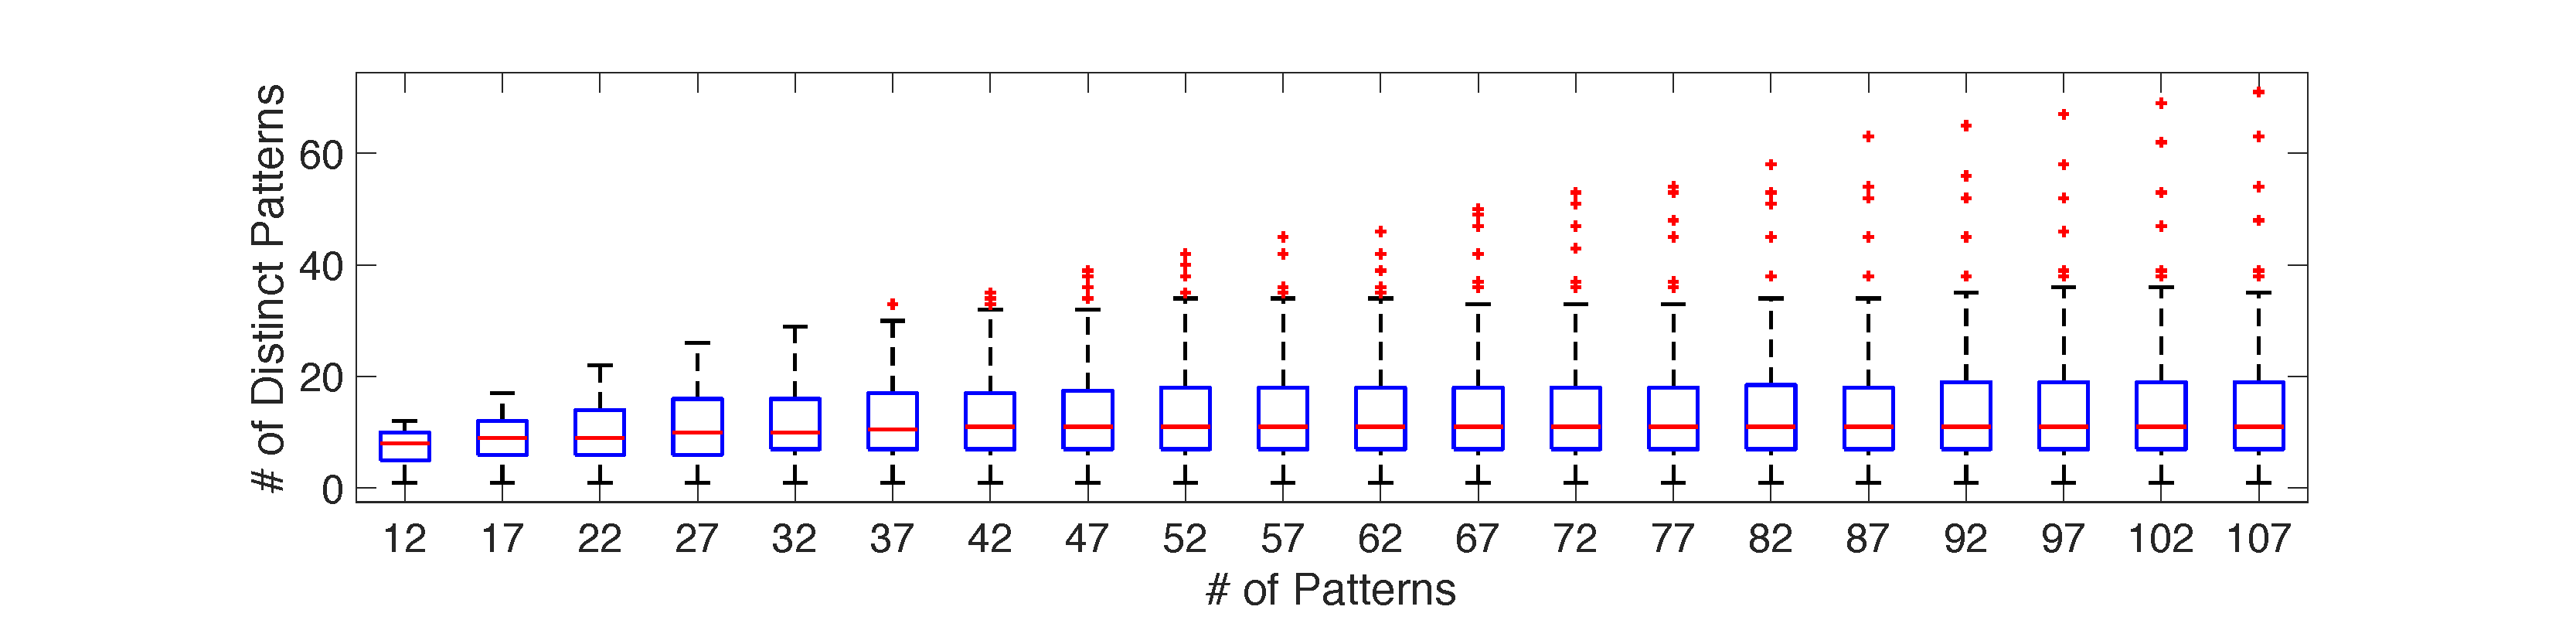
\includegraphics[width=\textwidth]{graphics/Laserlight_NumDistinctPatternsVNumPatterns.pdf}
% \bfcaption{Laserlight}      \label{fig:patterns_laserlight}
%\end{subfigure}
%    ~
%\begin{subfigure}[b]{0.48\textwidth}
%  \centering       
%  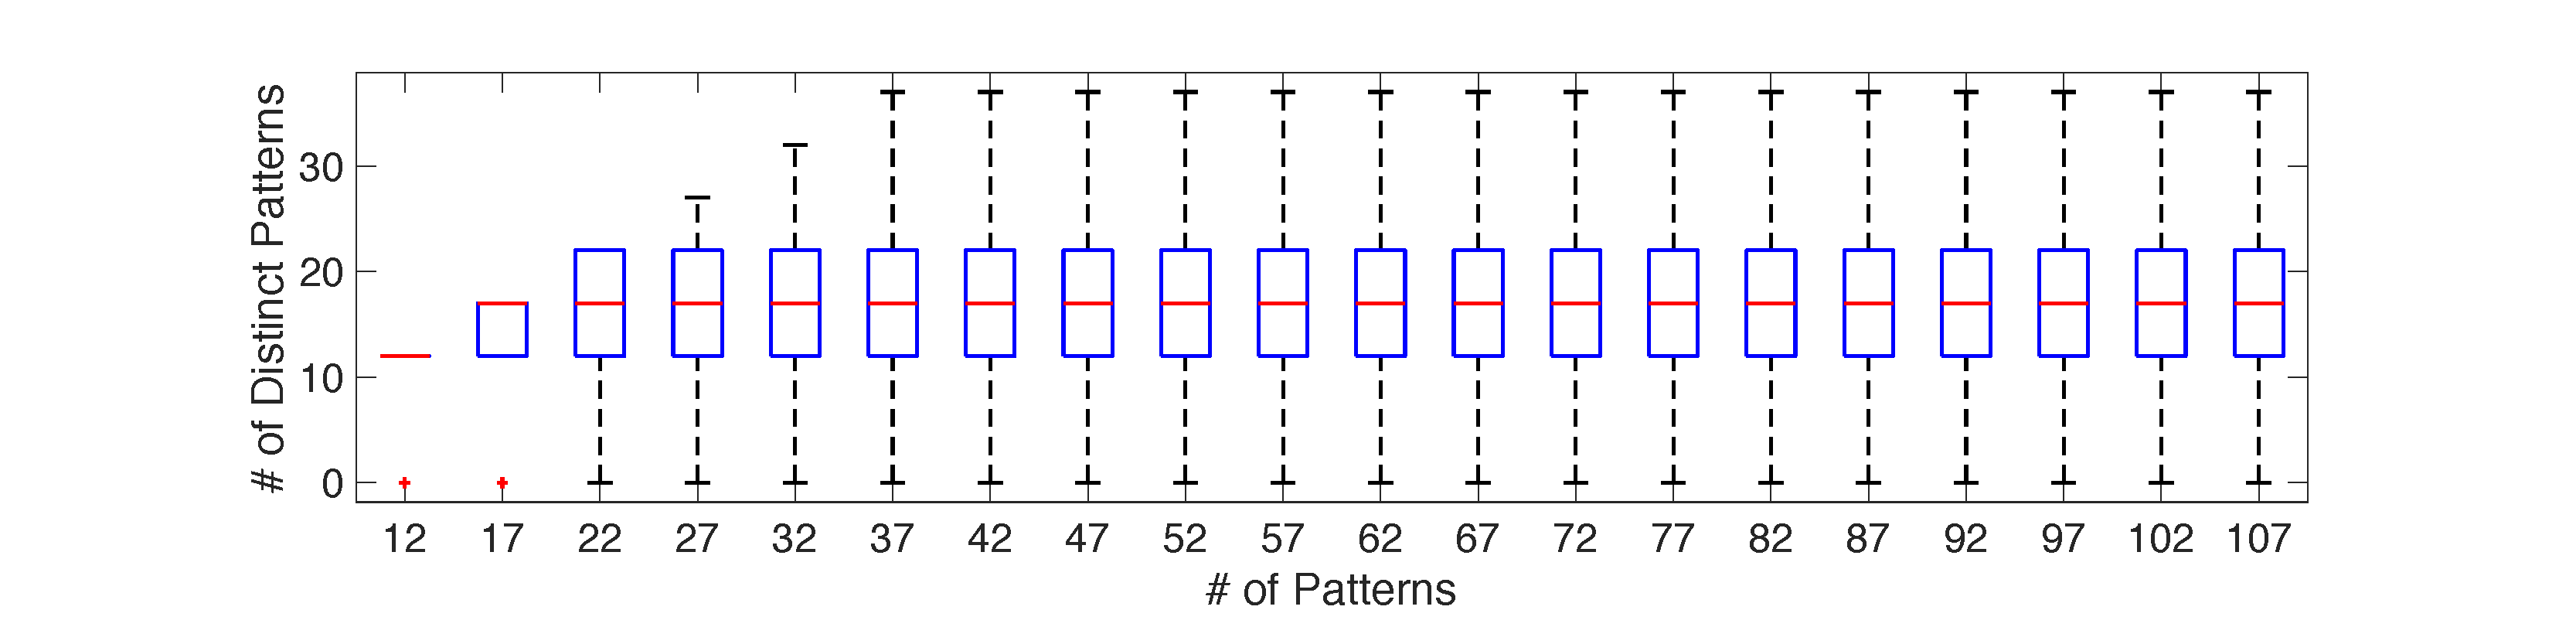
\includegraphics[width=\textwidth]{graphics/MTV_NumDistinctPatternsVNumPatterns.pdf}
% \bfcaption{MTV}     
% \label{fig:patterns_MTV}
%\end{subfigure}
%~
%\bfcaption{Distinct Patterns v. Number of Patterns }   \label{fig:distinctpatternsofpatternbasedalgorithms}
%\trimfigurewhitespace
%\end{figure}

%\tinysection{Pattern Diversification Failure}
%Recall in Section~\ref{sec:naivemixtureencodingrefinement} that pattern diversification can be time-consuming.
%As a result, both algorithms implement heuristics that sacrifice the capability of pattern diversification to some extent.
%In other words, increase in the total number of patterns mined from \textit{Laserlight} and \textit{MTV} may not lead to commensurate increase in the number of \textit{distinct} patterns (i.e., pattern duplication implies failure in pattern diversification).
%Specifically, we run \textit{MTV} and \textit{Laserlight} on each cluster ($30$ clusters in total) and vary the number of patterns configured for mining from $12$ to $107$.
%We collect the number of \textit{distinct} patterns that they have mined as well as the running time under each configuration.
%The experiment result is shown in Figure~\ref{fig:distinctpatternsofpatternbasedalgorithms} where y-axis is the number of distinct patterns and x-axis is the total number of patterns mined through \textit{Laserlight} and \textit{MTV}.
%We observe that \textit{Laserlight} and \textit{MTV} fail to extensively explore hidden feature-correlation in our chosen datasets.
%
%\begin{figure}[ht!]
%	\captionsetup[subfigure]{justification=centering}
%    \centering
%    \begin{subfigure}[b]{0.48\textwidth}
%        \centering       
%        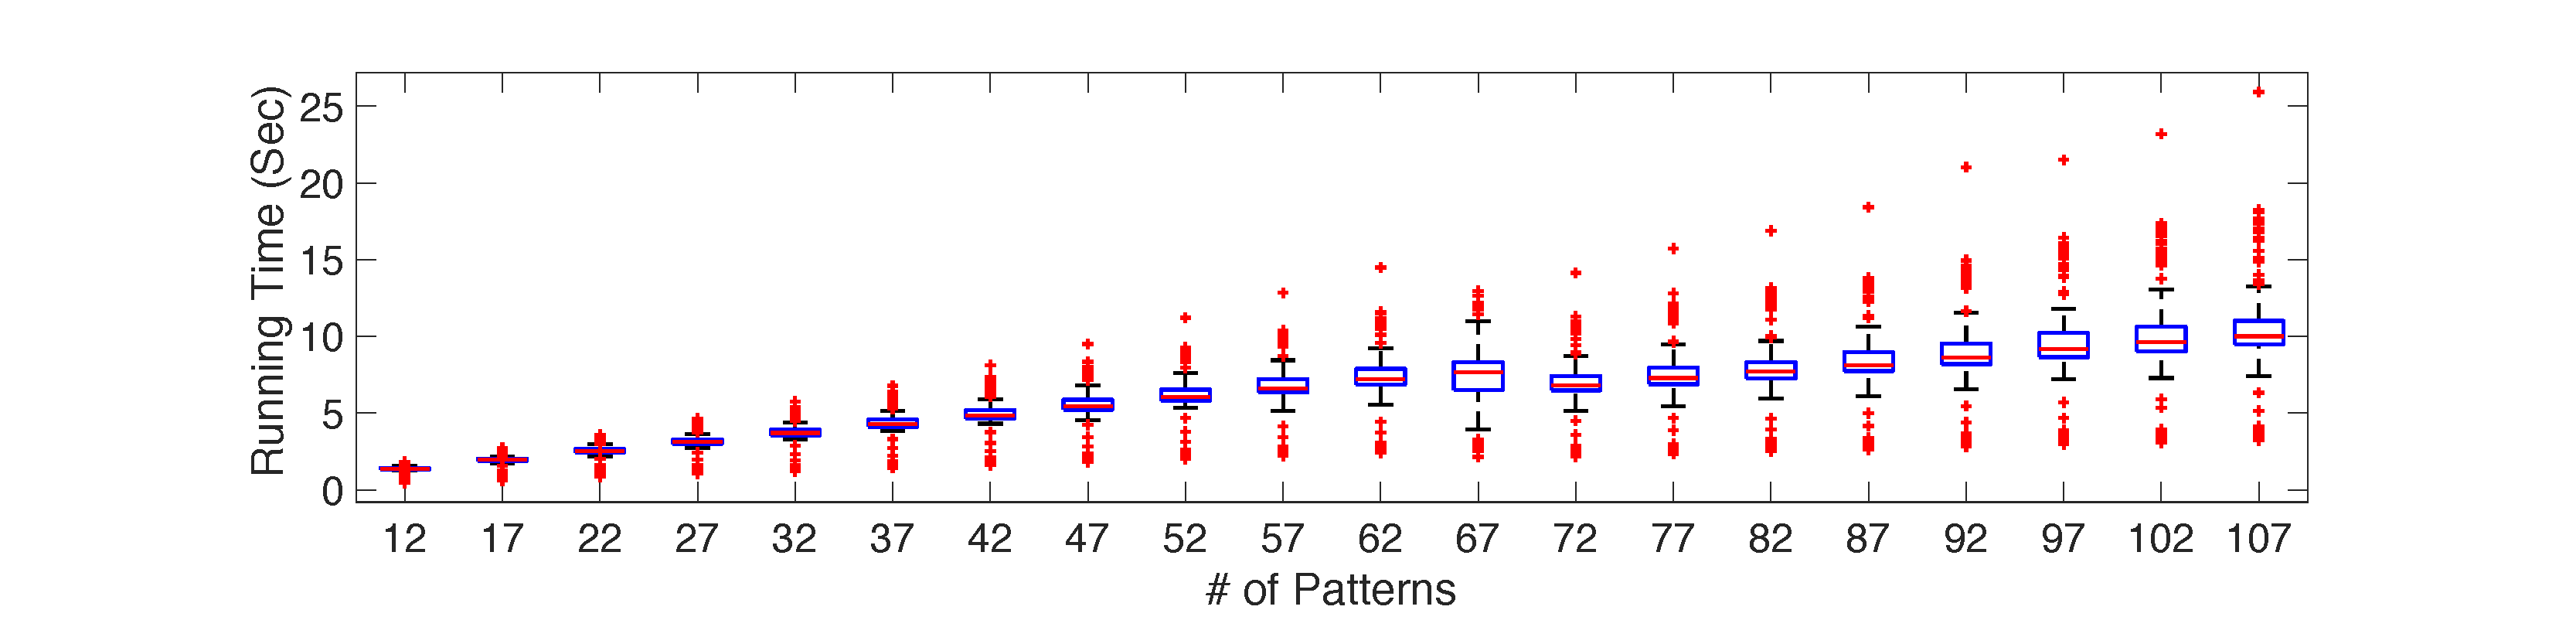
\includegraphics[width=\textwidth]{graphics/Laserlight_RunningTimeVNumPatterns.pdf}
% \bfcaption{Laserlight}      \label{fig:runningtime_laserlight}
%\end{subfigure}
%    ~
%\begin{subfigure}[b]{0.48\textwidth}
%  \centering       
%  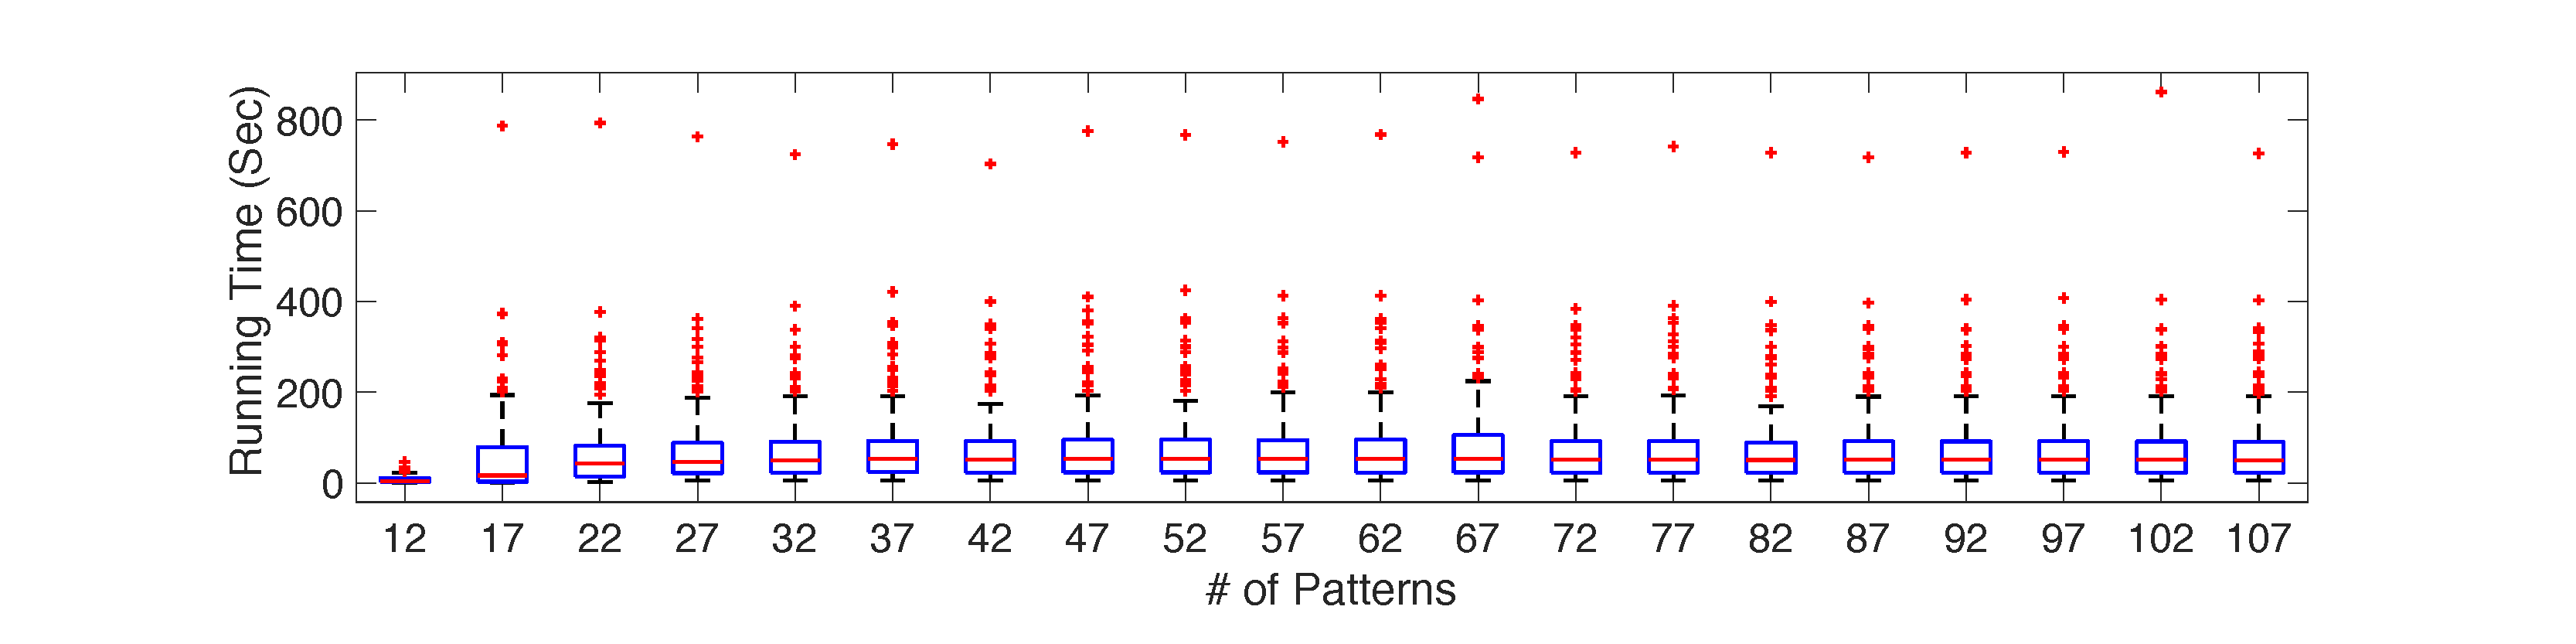
\includegraphics[width=\textwidth]{graphics/MTV_RunningTimeVNumPatterns.pdf}
% \bfcaption{MTV}     
% \label{fig:runningtime_MTV}
%\end{subfigure}
%~
%\bfcaption{Running Time v. Number of Patterns}   \label{fig:runningtimeofpatternbasedalgorithms}
%\trimfigurewhitespace
%\end{figure}
%
%\tinysection{Time Restriction}
%Computation efficiency will also influence effectiveness of pattern based summarizers when it takes too long to mine a potentially large set of informative patterns under from the data.
%The experiment result for running time analysis is shown in Figure~\ref{fig:runningtimeofpatternbasedalgorithms}.
%We observe that \textit{Laserlight} shows a close-to-linear growth rate.
%For \textit{MTV} the running time spikes at $17$ patterns and remains oscillating between high levels afterwards.
